% presentation source for the git-wizzard presentation
% build with the make file

\documentclass{beamer}
\mode<presentation>
\usetheme{Montpellier}
\usecolortheme{rose}

% preamble {{{

% packages {{{
\usepackage[normalem]{ulem}
\usepackage{listings}
% packages }}}

% defs {{{
\lstset{% set defaults
    basicstyle=\ttfamily,
    stringstyle=\ttfamily,
    showstringspaces=false
}
\lstnewenvironment{shell}
    {\lstset{language=sh}}
    {}
\hypersetup{% for links
    colorlinks,
    linkcolor=,
    urlcolor=blue
}
\theoremstyle{example}
\newtheorem{exercise}{Exercise}
\newcommand{\xkcd}[1]{\href{https://xkcd.com/#1}{xkcd/#1}}
% defs }}}

% metadata {{{
\title{Git Wizard 101}
\subtitle{Pearl Hacks}
% \author{D. Ben Knoble \\ \texttt{ben.knoble@gmail.com}}
\author{\href{https://benknoble.github.io}{D. Ben Knoble}}
% \urladdr[D. Ben Knoble]{https://benknoble.github.io} % or this
\institute{UNC Chapel Hill}
\date{23 February 2019}
% metadata }}}

% preamble }}}

\begin{document} % {{{

\frame{\titlepage}

\part{Getting Started}
\frame{\partpage}
\frame{\tableofcontents[part=1]}

\section{Ground Rules}
\begin{frame}{Ground Rules}
    \begin{itemize}
        \item Introduce yourself with name and pronouns
        \item Respect others' pronouns
        \item There are no dumb questions
        \item Help your neighbor when you can
        \item Have a good time!
    \end{itemize}
\end{frame}

\section{Introductions}
\begin{frame}{About Me}
    \begin{itemize}
        \item He/Him/His
        \item Senior (CS, French, Math), soon-to-be M.S. student
        \item \href{https://github.com/benknoble}{@benknoble} on GitHub
        \item<2-> Conversationally proficient in French, D\&D, puns
        \item<3-> And, of course, all things \texttt{git}
    \end{itemize}
\end{frame}

\begin{frame}{What We Will \emph{not} Be Doing}
    \begin{columns}
        \column{0.5\textwidth}
        \begin{figure}
            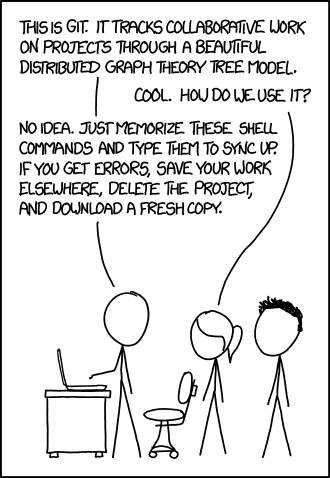
\includegraphics[scale=0.4]{img/git}
            \caption{\xkcd{1597}}
        \end{figure}

        \column{0.5\textwidth}
        \begin{itemize}
            \item Memorizing magic commands
            \item Learning the (beautiful) model behind \texttt{git}
        \end{itemize}
    \end{columns}
\end{frame}

% 
\includegraphics[scale=0.4]{img/documents}
% \caption{\xkcd{1459}}
% 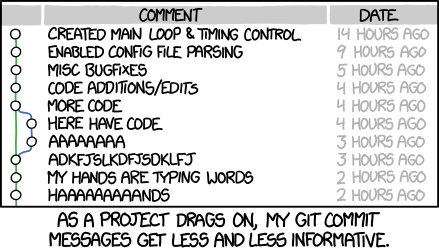
\includegraphics[scale=0.4]{img/git_commit}
% \caption{\xkcd{1296}}

\section{Setup}
\begin{frame}{Did You Get \texttt{git}?}
    Required setup
    \begin{enumerate}[<+->]
        \item
            \href{https://git-scm.com/book/en/v2/Getting-Started-Installing-Git}
            {\texttt{git}}
        \item
            \href{https://github.com}
            {GitHub account}
        \item \href{https://desktop.github.com}
            {GitHub Desktop}
        \item \href{https://github.com/benknoble/git-wizzard-code}
            {Forked starter code}
    \end{enumerate}
\end{frame}

\part{The Magic of \texttt{git}}
\frame{\partpage}
\frame{\tableofcontents[part=2]}

\section{Your First Commit}
\begin{frame}[fragile]{Lumos: Your First \sout{Spell} Commit}
    Not the time for \emph{commitment} problems
    \begin{exercise}[Make a commit]
        \begin{shell}
# this is the command-line version
git commit
        \end{shell}
    \end{exercise}
\end{frame}

\section{Experimentation}
\begin{frame}{Potions Class \& PPE\@: Experimenting Safely}
\end{frame}

\section{Collaboration}
\begin{frame}{Accio Code! Collaborating via Pull Requests}
\end{frame}

\section{{\textdagger}Merge Conflicts{\textdagger}}
\begin{frame}{Boggarts and Riddikulus: Merge Conflicts are \alert{not} Scary!}
\end{frame}

\part{Conclusion}
\begin{frame}{Conclusion}
    \begin{block}{Who Am I?}
    \end{block}
    \begin{block}{Summary}
    \end{block}
    \begin{block}{Resources}
    \end{block}
    \begin{block}{Reminders}
    \end{block}
    \begin{block}{Upcoming Wizard Classes}
    \end{block}
\end{frame}

% \appendix

\end{document} % }}}
